\documentclass[12pt]{article}
\usepackage[margin=1in]{geometry} % For setting margins
\usepackage{graphicx} % For including images
\usepackage{hyperref} % For hyperlinks
\usepackage{fontspec} % Allows for system fonts
\usepackage{fancyhdr} % Add this for header and footer customization
\usepackage{parskip} % Handles paragraph spacing instead of indentation
\usepackage{xcolor}
\usepackage{booktabs} % For formal tables
\usepackage{array} % For specifying column formats
\usepackage{longtable} % For tables that span multiple pages
\usepackage{pdfpages}

% Define custom color with transparency
\definecolor{headerfooterGray}{gray}{0.5} % Change gray to any color you prefer
\newcommand{\transparenttext}[1]{{\special{pdf:literal 0.5 Tr}#1\special{pdf:literal 0 Tr}}}

% Increases the spacing between all rows by 50%
\renewcommand{\arraystretch}{1.5}

% Set document font to Avenir Next LT Pro
\setmainfont{Avenir Next LT Pro} % This requires the font to be installed on your system

\setlength{\parskip}{0.75em} % Adjust the space between paragraphs as needed

\pagestyle{fancy}
\fancyhf{} % Clear default header and footer settings
\lhead{\textcolor{headerfooterGray}{\transparenttext{Edgar Ulmer}}} % Your name in the left header with transparency
\rfoot{\textcolor{headerfooterGray}{\transparenttext{\thepage}}} % Page number in the left footer with transparency
\renewcommand{\headrulewidth}{0pt}
\renewcommand{\footrulewidth}{0pt}

\title{Comprehensive Exam for Senior Film Majors\\Spring 2024}
\author{Pseudonym: Edgar Ulmer}
\date{\today}

\begin{document}

\maketitle

\thispagestyle{empty}

\section*{Part 1: The Sequence Analysis}

“Do the Right Thing” (1989) - Racist Stereotypes

In this sequence from Spike Lee's "Do the Right Thing," cinematography, narrative structure, and race consciousness synergizes to render a contentiuos moment and to deliver a creative fourth wall break. This part of the movie, which starts with a camera shot over Mookie's shoulder, pulls the viewer right into Mookie's world, making it clear that this moment is from his viewpoint. This is crucial because it not only makes the audience see things from Mookie's perspective but also sets them up to think deeply about the conversation that follows between Mookie and Pino about their favorite celebrities.

Lee's choice to frame Mookie and Pino together in the same shot as they discuss this topic is intentional. It visually emphasizes the clash between their views, representing racial divides. Mookie's face is lit more brightly than Pino's  physically highlighting Mookie but also positioning him as the moral center of this conversation. Because of Lee's intention to connect with black audience's experiences and to challenge Racism from a black perspective, the sequence emphasizes empathy for Mookie's perspective.

The scene peaks with a sequence where different characters look straight into the camera to deliver racial slurs. Similair to other expositional moments in the film, the montage directly involves the audience in the film's examination of racism. This montage ellicits a strong emotional response, and Lee is challenging viewers to face their own biases and the widespread nature of racism.

The sequence is put together to demonstrates Lee's deep understanding of how to use film to communicate complex issues. By placing a racialy charged interaction against an unblinking visual montage of racial conflict, Lee highlights how deeply embedded racism is in everyday life and across the fabric of society through implicating us in outburts of racist rage.

Analyzing the specific sequence from "Do the Right Thing" through the perspectives of Jerome Christensen and W. J. T. Mitchell provides a nuanced understanding of the film's engagement with race and racism. Christensen's critique positions Spike Lee's work within the context of corporate influence, arguing that the film, while ostensibly exploring racial identity, ultimately succumbs to the forces of consumerism​​. This viewpoint suggests that the montage, rather than being purely an artistic expression of racial tensions, might also serve to commodify those tensions, packaging them in a manner palatable and marketable within the broader scope of American consumer culture.

Conversely, Mitchell's analysis praises the film for its public art virtues, highlighting its ability to stimulate societal discourse on pivotal issues like race, class, and consumer capitalism​​. This perspective valorizes the direct-to-camera montage as a powerful tool for societal reflection, urging viewers to confront the pervasive and systemic nature of racism. Mitchell perceives the film as a catalyst for dialogue and change, an embodiment of public art that transcends mere entertainment to probe deeply into the racial divides and the complexities surrounding them.

Re-evaluating the sequence through these lenses, the montage emerges as a multifaceted cinematic device. On one hand, following Christensen's argument, one could interpret the sequence as leveraging racial conflict as a means of engaging audiences in a manner that aligns with the interests of the film industry's corporate stakeholders. This interpretation suggests a potential dilution of the film's racial commentary through its entanglement with commercial objectives, casting a shadow on the sequence's authenticity as a critique of racism.

On the other hand, Mitchell's perspective offers a counterpoint, framing the montage as a deliberate, confrontational strategy employed by Lee to force viewers to reckon with the uncomfortable realities of racism. From this viewpoint, the sequence is not merely a narrative technique but a radical act of public art, transforming the theatre into a space for confronting societal ills. This reading aligns the montage with Lee's broader intent to provoke, challenge, and ultimately spark discourse on race relations in America.

In synthesizing these analyses, the montage at the heart of "Do the Right Thing" can be seen as embodying both the potential pitfalls of navigating racial discourse within a commercial framework, as highlighted by Christensen, and the powerful capacity of film to serve as a medium for social commentary and change, as emphasized by Mitchell. Thus, the sequence stands as a testament to Lee's innovative  negotiation of artistic expression, racial politics, and the commercial realities of filmmaking, challenging audiences to engage with the layered and contentious realities of race in America.

\clearpage

\begin{thebibliography}{5}

\bibitem{christensen1991}
Jerome Christensen,
``Spike Lee, Corporate Populist,''
\textit{Critical Inquiry},
vol. 17, no. 3, 1991, pp. 582–595.

\bibitem{cooper1998}
Brenda Cooper,
``‘The White-Black Fault Line’: Relevancy of Race and Racism in Spectators’ Experiences of Spike Lee’s Do the Right Thing,''
\textit{Howard Journal of Communications},
vol. 9, no. 3, July 1998, pp. 205–228,
\url{https://doi.org/10.1080/106461798246998}.

\bibitem{johnson2017}
Brian C. Johnson,
``Baltimore 2015, Black Lives Matter and the Prescience of Spike Lee’s Do the Right Thing,''
\textit{Film International (16516826)},
vol. 15, no. 1, March 2017, pp. 23–36,
\url{https://doi.org/10.1386/fiin.15.1.23_1}.

\bibitem{mitchell1991}
W. J. T. Mitchell,
``Seeing ‘Do the Right Thing’,''
\textit{Critical Inquiry},
vol. 17, no. 3, 1991, pp. 596–608.

\bibitem{linguistics2002}
``The Linguistics of Color Blind Racism: How to Talk Nasty about Blacks without Sounding ‘Racist’,''
Accessed April 8, 2024,
\url{https://doi.org/10.1177/08969205020280010501}.

\end{thebibliography}

\newpage

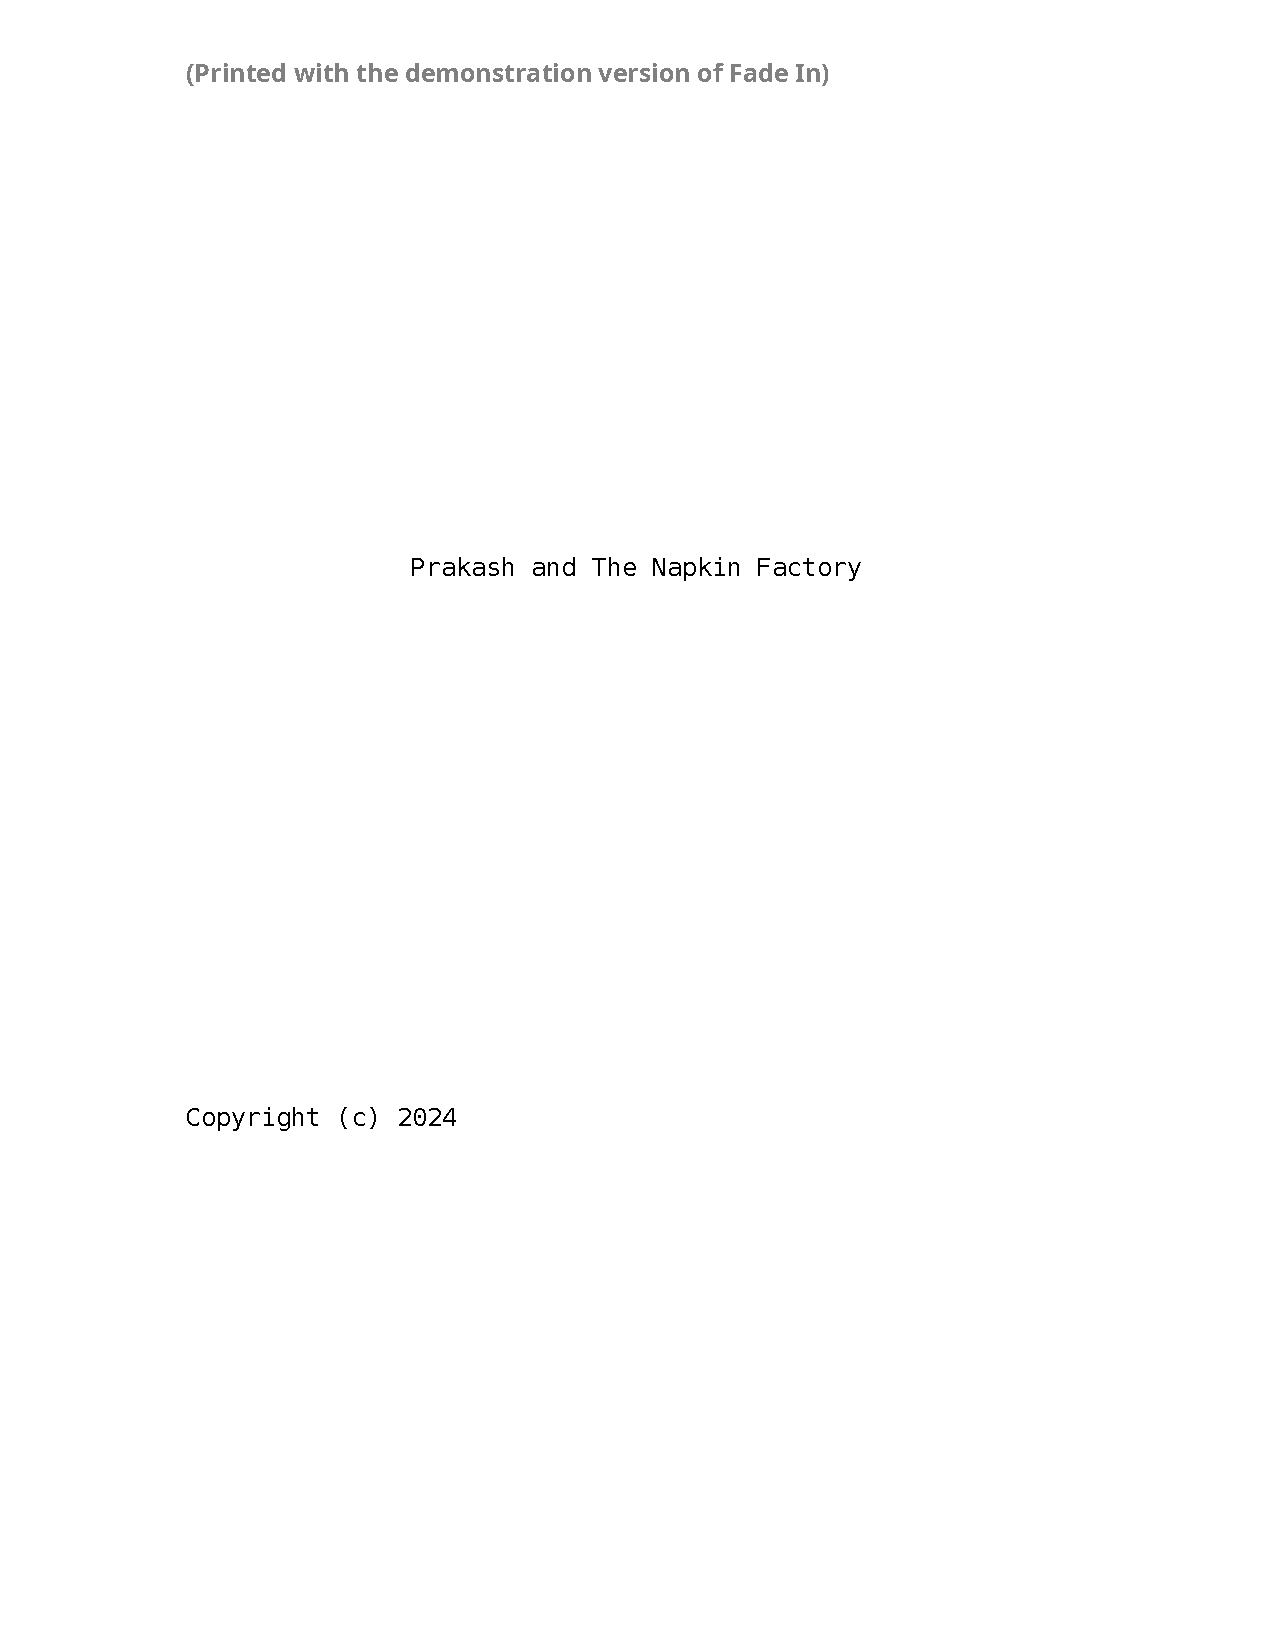
\includepdf[pages=-, scale=.8, pagecommand=\section*{Part 2: Screenwriting Prompt}]{./prakash-and-the-napkin-factory.pdf}

\newpage

\section*{Part 3: Directing Exercise}

This scene unfolds in a cozy, crowded restaurant, transitioning from a light-hearted dinner to a more somber tone with Miles's phone call to Victoria. The cinematography will focus heavily on delivering the nuance of the characters' interactions, the atmospheric conditions of the restaurant, and the internal turmoil of Miles. The dinner scene will be treated with warmth and familiarity, employing softer lighting and a mix of static and dynamic shots to emphasize the camaraderie and underlying tensions. In contrast, Miles's phone call will utilize more isolated framing and darker lighting to reflect his emotional isolation and the distressed nature of the conversation.

\subsection*{Cinematography Style}

Adhering to a Hitchcockian "pure cinema" approach blended with dynamic framing reminiscent of early 2000s television, the cinematography will focus on visual storytelling through movement, composition, and perspective. Wide lenses will be used for establishing shots and group dynamics, while longer lenses will isolate characters during moments of personal reflection or intense interaction. The camera work will shift from static to moving shots, employing handheld or steadicam techniques to enhance the emotional resonance of key moments.


\subsection*{Directorial Approach}

To direct this scene in 'Sideways', I would emply the camera as an active agent in the narrative. The camera movements would be deliberate, with steadicam shots for entering the restaurant to convey a sense of immersion into the scene, and a head mount for Miles's anxiety attack to reflect his disorientation and distress. The use of close-ups is strategic, aiming to capture the raw emotions and subtle nuances of the characters' interactions.

The scene transitions are fluid, with each shot designed to lead into the next seamlessly, maintaining the narrative's rhythm while also allowing for moments of introspection. I will lean into the power of dramatic lighting, with emphasis on natural lighting for the more intimate moments to accentuate warmth and connection, contrasted with harsher shadows during Miles's phone call to highlight his heartbreak.

In sum, this directorial vision aims to convey the contours of each character with a visually engaging narrative, utilizing innovative blocking and camera work to render the subtextual nuances of human conversation. The scene's treatment is carefully crafted to maintain a balance between the external environment and the characters' internal worlds.


\vspace{70pt} 

\subsection*{Shot List} 

{\fontsize{8}{10}\selectfont % Making the table font size smaller
\begin{longtable}{>{\raggedright\arraybackslash}p{1.7cm} >{\raggedright\arraybackslash}p{1.5cm} >{\raggedright\arraybackslash}p{0.5cm} >{\raggedright\arraybackslash}p{4.7cm} >{\raggedright\arraybackslash}p{2cm} >{\raggedright\arraybackslash}p{1.5cm} >{\raggedright\arraybackslash}p{1.5cm}}
\toprule
\textbf{EXT / INT} & \textbf{Location} & \textbf{\#} & \textbf{Shot Description} & \textbf{Camera Movement} & \textbf{Lens (MM)} & \textbf{Angle} \\
\midrule
INT & MATTEI’S TAVERN & 1 & Entrance of Miles and Jack, greeted by the hostess & Static & 24mm & Medium \\
INT & MATTEI’S TAVERN & 2 & Maya and Stephanie waving from the booth & OTS & 85mm & Medium \\
INT & MATTEI’S TAVERN & 3 & Jack and Miles approaching the table, Jack's confident stride & Tracking & 35mm & Long \\
INT & MATTEI’S TAVERN & 4 & Two Shot. Jack sitting next to Stephanie, hand on her neck & Static & 50mm & Medium \\
INT & MATTEI’S TAVERN & 5 & Two shot. Miles asking Maya about her drink & Static & 50mm & Medium \\
INT & MATTEI’S TAVERN & 6 & Miles tasting the wine, beginning to relax & Static & 85mm & Close-up \\
INT & MATTEI’S TAVERN & 7 & Waiter describing specials to the group & Steadicam, circling table & 24mm & Medium \\
INT & MATTEI’S TAVERN & 8 & Miles raising hand for wine list, then passing it & Cut to & 35mm & Medium \\
INT & MATTEI’S TAVERN & 9 & Stephanie scanning wine menu, decision-making & Pan & 50mm & Close-up (Menu) to Medium (Stephanie) \\
INT & MATTEI’S TAVERN & 10 & Group's reaction to "Pinot Noir" decision, high-five & Static & 24mm & Medium \\
INT & MATTEI’S TAVERN & 11 & Arrival of the first wine, opening and pouring & Static & 85mm & Close-up \\
INT & MATTEI’S TAVERN & 12 & Group enjoying dinner, laughter and conversation & Handheld, moves between speakers, and plates arriving & 80mm & Close-up \\
INT & MATTEI’S TAVERN & 13 & Miles's growing intoxication, Jack's concern & Series of Close-ups & Varied, 50mm to 85mm & Mixed Angles \\
INT & MATTEI’S TAVERN & 14 & Jack stopping Miles from pouring more wine & Close-up (Hands) & 85mm & High Angle \\
INT & MATTEI’S TAVERN & 15 & Close on Miles as anxiety builds & Static & 85mm & Close-up \\
INT & UNDERWORLD & 16 & Miles boarding boat on River Styx, Charon in background & Dolly in & 35mm & Wide \\
INT & MATTEI’S TAVERN & 17 & Miles snaps back to reality, observing Jack and Stephanie & Static & 50mm & Medium \\
INT & MATTEI’S TAVERN & 18 & Maya conversing with a disoriented Miles & Over-the-Shoulder & 85mm & Close-up \\
INT & MATTEI’S TAVERN & 19 & '96 Comte Armand Pommard brought to the table & Static & 50mm & Medium Shot \\
INT & MATTEI’S TAVERN & 20 & Jack and Stephanie share a kiss & Close-up & 85mm & Eye Level \\
INT & MATTEI’S TAVERN & 21 & Miles navigating to the bathrooms, unsteady & Handheld & 24mm & POV6 \\
INT & MATTEI’S TAVERN & 22 & Miles attempts the Men’s room, then takes Xanax & Static & 50mm & Medium Close-up \\
INT & MATTEI’S TAVERN & 23 & Miles dials phone, numbers and tones out of sync & Close-up & 50mm & High Angle \\
INT & MATTEI’S TAVERN & 24 & Close on Miles during phone conversation with Victoria & Static & 85mm & Close-up \\
EXT & DEEP CANYON  & 25 & Miles on rope bridge across chasm (Flash scene) & Dolly out & 24mm & Wide \\
INT & MATTEI’S TAVERN & 26 & Miles slips onto the floor trying to sit & High Angle & 35mm & Wide \\
\bottomrule
\end{longtable}
}

\vspace{-15pt} 
\newpage

\section*{Part 4: Editing Exercise}
% Content here

\textbf{\href{https://drive.google.com/file/d/1EqL9ED4QaTvNsAf8bgZrvc-a0rlqhiv3/view?usp=sharing }{Click here to access my edited version of "Horizon"}}

\end{document}
